\clearpage
\begin{textbox}{\href{https://compneuro.neuromatch.io/tutorials/W3D1_BayesianDecisions/student/W3D1_Tutorial1.html}{Bayes with a binary hidden state } }
\begin{subbox}{subbox}{Introduction}
\scriptsize

We will introduce the fundamental building blocks for Bayesian statistics: 

1. How do we combine the possible loss (or gain) for making a decision with our probabilistic knowledge?\\
2. 
 How do we use probability distributions to represent hidden states?\\
3. How does marginalization work and how can we use it?\\
 4. How do we combine new information with our prior knowledge? 

\end{subbox}

\begin{subbox}{subbox}{Gone Fishin'}
\scriptsize
We are going to explore \textbf{binary hidden state problem} by going fishing. We need to decide which side to fish on--the hidden state. We know fish like to school together. On different days the school of fish is either on the left or right side, but we don’t know what the case is today. We define our knowledge about the fish location as a distribution over the random hidden state variable. Using our probabilistic knowledge, also called our \textbf{belief} about the hidden state, we will explore how to make the decision about where to fish today, based on what to expect in terms of gains or losses for the decision.
The gains and loss are defined by the utility of choosing an action, which is fishing on the left or right. 

\end{subbox}
\begin{subbox}{subbox}{Deciding where to fish}
\scriptsize

Let's start to get a sense of how all this works using an example. First, make sure we understand how the expected utility of each action is being computed from the probabilities and the utility values. In the initial state: the probability of the fish being on the left is 0.9 and on the right is 0.1. The expected utility of the action of fishing on the left is then $U(s = \textrm{left},a = \textrm{left})p(s = \textrm{left}) + U(s = \textrm{right},a = \textrm{left})p(s = \textrm{right}) = 2(0.9) + -2(0.1) = 1.6$. Essentially, to get the expected utility of action $a$, we are doing a weighted sum over the relevant column of the utility matrix (corresponding to action $a$) where the weights are the state probabilities.

\centering
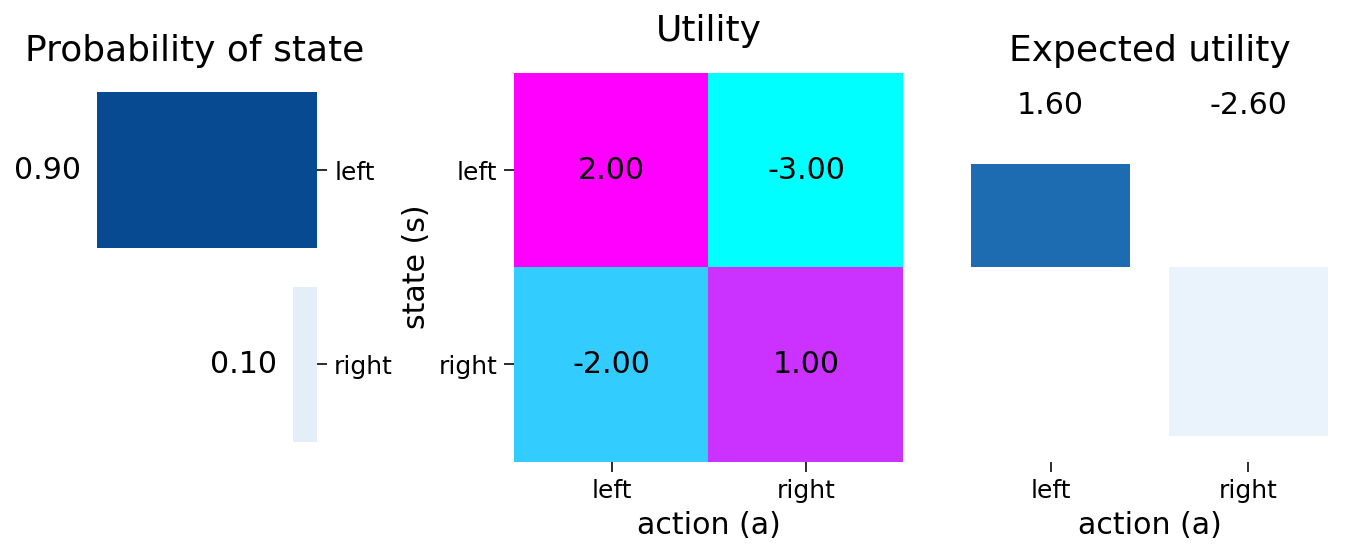
\includegraphics[scale=0.23]{Figures/BD/BD_Figure1.png}

\end{subbox}
\end{textbox}
%%%%%%%%%%%%%%%%%%%%%%%%%%%%%%%%%%%%%%%%%%%%%%%%%%
%%%%%%%%%%%%%%%%%%%%%%%%%%%%%%%%%%%%%%%%%%%%%%%%%%
\begin{textbox}{\href{https://compneuro.neuromatch.io/tutorials/W3D1_BayesianDecisions/student/W3D1_Tutorial1.html}{Bayes with a binary hidden state } }
\begin{subbox}{subbox}{Likelihood of the fish being on either side}
\scriptsize

First, we'll think about what it means to take a measurement (also often called an observation or just data) and what it tells us about what the hidden state may be. Specifically, we'll be looking at the \textbf{likelihood}, which is the probability of our measurement ($m$) given the hidden state ($s$): $P(m | s)$. Remember that in this case, the hidden state is which side of the dock the school of fish is on.
We will watch someone fish (for let's say 10 minutes) and our measurement is whether they catch a fish or not. We know something about what catching a fish means for the likelihood of the fish being on one side or the other.

\end{subbox}

\begin{subbox}{subbox}{Guessing the location of the fish}
\scriptsize
Let's say we go to a different dock to fish. Here, there are different probabilities of catching fish given the state of the world. At this dock, if we fish on the side of the dock where the fish are, we have a 70\% chance of catching a fish. If we fish on the wrong side, we will catch a fish with only 20\% probability. These are the likelihoods of observing someone catching a fish! That is, we are taking a measurement by seeing if someone else catches a fish!

\textit{We see a fisher-person is fishing on the left side.}
 
In the example, we tried to guess where the school of fish was based on the measurement we took (watching someone fish). We did this by choosing the state (side where we think the fish are) that maximized the probability of the measurement. In other words, we estimated the state by maximizing the likelihood (the side with the highest probability of measurement given state $P(m|s$)). This is called maximum likelihood estimation (MLE).

But, what if we had been going to this dock for years and we knew that the fish were almost always on the left side? This should probably affect how we make our estimate -- we would rely less on the single new measurement and more on our prior knowledge. This is the fundamental idea behind Bayesian inference.

\end{subbox}

\end{textbox}
%%%%%%%%%%%%%%%%%%%%%%%%%%%%%%%%%%%%%%%%%%%%%%%%%%
%%%%%%%%%%%%%%%%%%%%%%%%%%%%%%%%%%%%%%%%%%%%%%%%%%
\begin{textbox}{\href{https://compneuro.neuromatch.io/tutorials/W3D1_BayesianDecisions/student/W3D1_Tutorial1.html}{Bayes with a binary hidden state } }
\begin{subbox}{subbox}{Correlation}
\scriptsize

We are going to take a step back for a bit and think more generally about the amount of information shared between two random variables. We want to know how much information we gain when we observe one variable (take a measurement) if we know something about another. We will see that the fundamental concept is the same if we think about two attributes, for example the size and color of the fish, or the prior information and the likelihood.

\end{subbox}
\begin{subbox}{subbox}{Covarying probability distributions
}
\scriptsize

The relationship between the marginal probabilities and the joint probabilities is determined by the correlation between the two random variables - a normalized measure of how much the variables covary. We can also think of this as gaining some information about one of the variables when we observe a measurement from the other.  

Here, we want to think about how the correlation between size and color of these fish changes how much information we gain about one attribute based on the other. 

\centering
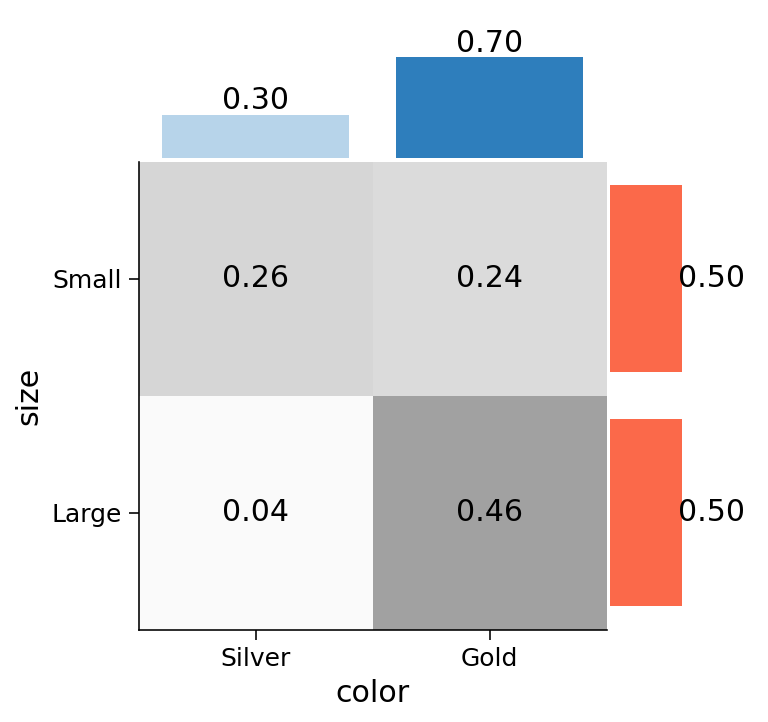
\includegraphics[scale=0.35]{Figures/BD/BD_Figure2.png}

\end{subbox}


\end{textbox}
%%%%%%%%%%%%%%%%%%%%%%%%%%%%%%%%%%%%%%%%%%%%%%%%%%
%%%%%%%%%%%%%%%%%%%%%%%%%%%%%%%%%%%%%%%%%%%%%%%%%%

\begin{textbox}{\href{https://compneuro.neuromatch.io/tutorials/W3D1_BayesianDecisions/student/W3D1_Tutorial1.html}{Bayes with a binary hidden state } }
\begin{subbox}{subbox}{Marginalisation}
\scriptsize
We may want to find the probability of one variable while ignoring another: we will do this by averaging out, or marginalizing, the irrelevant variable.

We will think of this in two different ways.

In the first math exercise, we will think about the case where we know the joint probabilities of two variables and want to figure out the probability of just one variable. To make this explicit, let's assume that a fish has a color that is either gold or silver (our first variable) and a size that is either small or large (our second). We could write out the the \textbf{joint probabilities}: the probability of both specific attributes occuring together. For example, the probability of a fish being small and silver, $P(X = \textrm{small}, Y = \textrm{silver})$, is 0.4. The following table summarizes our joint probabilities:

\begin{center}
\begin{tabular}{||c c c||} 
 \hline
 P(X, Y) & Y = silver & Y = gold \\ [0.5ex] 
 \hline\hline
 X = small & 0.4 & 0.2\\ 
 \hline
 X = large & 0.1  & 0.3  \\ [1ex] 
 \hline
\end{tabular}
\end{center}
We want to know what the probability of a fish being small  regardless of color. Since the fish are either silver or gold, this would be the probability of a fish being small and silver plus the probability of a fish being small and gold. This is an example of marginalizing, or averaging out, the variable we are not interested in across the rows or columns.. In math speak: $P(X = \textrm{small}) = \sum_y{P(X = \textrm{small}, Y)}$. This gives us a \textbf{marginal probability}, a probability of a variable outcome (in this case size), regardless of the other variables (in this case color).

More generally, we can marginalize out a second irrelevant variable $y$ by summing over the relevant joint probabilities:

$$p(x) = \sum_y p(x, y) $$

To find the marginal probability of a measurement we will remove an unknown (the hidden state). We will do this by marginalizing out the hidden state. In this case, we know the conditional probabilities of the measurement given state and the probabilities of each state. We can marginalize using:

$$p(m) = \sum_s p(m | s) p(s) $$

These two ways of thinking about marginalization (as averaging over joint probabilities or conditioning on some variable) are equivalent because the joint probability of two variables equals the conditional probability of the first given the second times the marginal probability of the second:

$$p(x, y) = p(x|y)p(y)$$ 


\end{subbox}

\end{textbox}
%%%%%%%%%%%%%%%%%%%%%%%%%%%%%%%%%%%%%%%%%%%%%%%%%%
%%%%%%%%%%%%%%%%%%%%%%%%%%%%%%%%%%%%%%%%%%%%%%%%%%
\begin{textbox}{\href{https://compneuro.neuromatch.io/tutorials/W3D1_BayesianDecisions/student/W3D1_Tutorial1.html}{Bayes with a binary hidden state } }
\begin{subbox}{subbox}{Computing marginal probabilities}
\scriptsize

 The probability of a fish being silver is the joint probability of it being
     small and silver plus the joint probability of it being large and silver:
\begin{eqnarray*}
 P(Y = silver) =\\ 
 P(X = small, Y = silver) + P(X = large, Y = silver)\\
                  = 0.4 + 0.1
                  = 0.5
                  \end{eqnarray*} 
This is all the possibilities as in this scenario, our fish can only be small
   or large, silver or gold. So the probability is 1 - the fish has to be at
   least one of these.\\
 First we compute the marginal probabilities
\begin{align*} P(X = small) =\\ P(X = small, Y = silver) + P(X = small, Y = gold)\\ = 0.4+0.2=0.6\end{align*} 
\begin{align*}  P(Y = gold) = \\P(X = small, Y = gold) + P(X = large, Y = gold) = 0.5\end{align*} 
   We already know the joint probability: \begin{align*} P(X = small, Y = gold) = 0.2\end{align*} 
   We can now use the given formula:
\begin{align*}    P( X = small or Y = gold) = \\P(X = small) + P(Y = gold) - P(X = small, Y = gold)\\
                             = 0.6 + 0.5 - 0.2
                             = 0.9 \end{align*} 
                             
                    

\end{subbox}
\begin{subbox}{subbox}{Computing marginal likelihood}
\scriptsize
When we normalize to find the posterior, we need to determine the marginal likelihood--or evidence--for the measurement we observed. To do this, we need to marginalize as we just did above to find the probabilities of a color or size. Only, in this case, we are marginalizing to remove a conditioning variable! In this case, let's consider the likelihood of fish (if we observed a fisher-person fishing on the \textit{right}).

\begin{center}
\begin{tabular}{||c c c||} 
 \hline
 p(m\|s)  & m = fish & m = no fish \\ [0.5ex] 
 \hline\hline
s = left & 0.1 & 0.9\\ 
 \hline
s = right & 0.5  & 0.5  \\ [1ex] 
 \hline
\end{tabular}
\end{center}
The table above shows us the \textbf{likelihoods}, just as we explored earlier.

We want to know the total probability of a fish being caught, $P(m = \textrm{fish})$, by the fisher-person fishing on the right. (We would need this to calculate the posterior.) To do this, we will need to consider the prior probability, $p(s)$, and marginalize over the hidden states!

This is an example of marginalizing, or conditioning away, the variable we are not interested in as well.


\end{subbox}

\end{textbox}
%%%%%%%%%%%%%%%%%%%%%%%%%%%%%%%%%%%%%%%%%%%%%%%%%%
%%%%%%%%%%%%%%%%%%%%%%%%%%%%%%%%%%%%%%%%%%%%%%%%%%
\begin{textbox}{\href{https://compneuro.neuromatch.io/tutorials/W3D1_BayesianDecisions/student/W3D1_Tutorial1.html}{Bayes with a binary hidden state } }
\begin{subbox}{subbox}{Computing marginal likelihood}
\scriptsize

Given the priors
Priors
$$P(s = left) = 0.3$$
$$P(s = right) = 0.7$$
and the likelihoods
$$P(m = fish | s = left) = 0.1$$
$$P(m = fish | s = right) = 0.5$$
$$P(m = no fish | s = left) = 0.9$$
$$P(m = no fish | s = right) = 0.5$$

We can calculate the marginal likelihood (evidence):
 \begin{eqnarray*}   P(m = fish)\\ 
 = P(m = fish, s = left) + P(m = fish, s = right)\\
                = P(m = fish | s = left)P(s = left) +\\ P(m = fish | s = right)P(s = right)\\
                = 0.1 * 0.3 + .5 * .7
            = 0.38
            \end{eqnarray*}
We can calculate the marginal likelihood (evidence): 
  \begin{eqnarray*}    P(m = fish) =\\ P(m = fish, s = left) + P(m = fish, s = right)
                =\\ P(m = fish | s = left)P(s = left) + \\P(m = fish | s = right)P(s = right)\\
                = 0.1 * 0.6 + .5 * .4
                = 0.26
                 \end{eqnarray*} 
\end{subbox}

\end{textbox}
%%%%%%%%%%%%%%%%%%%%%%%%%%%%%%%%%%%%%%%%%%%%%%%%%%
%%%%%%%%%%%%%%%%%%%%%%%%%%%%%%%%%%%%%%%%%%%%%%%%%%
\begin{textbox}{\href{https://compneuro.neuromatch.io/tutorials/W3D1_BayesianDecisions/student/W3D1_Tutorial1.html}{Bayes with a binary hidden state } }
\begin{subbox}{subbox}{Bayes' Rule and the Posterior}
\scriptsize
Marginalization is going to be used to combine our prior knowledge, which we call the \textbf{prior}, and our new information from a measurement, the \textbf{likelihood}. Only in this case, the information we gain about the hidden state we are interested in, where the fish are, is based on the relationship between the probabilities of the measurement and our prior. 

We can now calculate the full posterior distribution for the hidden state ($s$) using Bayes' Rule. As we've seen, the posterior is proportional to the prior times the likelihood. This means that the posterior probability of the hidden state ($s$) given a measurement ($m$) is proportional to the likelihood of the measurement given the state times the prior probability of that state:

\begin{equation}
P(s | m) \propto P(m | s) P(s)
\end{equation}

We say proportional to instead of equal because we need to normalize to produce a full probability distribution:

\begin{equation}
P(s | m) = \frac{P(m | s) P(s)}{P(m)}
\end{equation}

Normalizing by this $P(m)$ means that our posterior is a complete probability distribution that sums or integrates to 1 appropriately. We now can use this new, complete probability distribution for any future inference or decisions we like! In fact, as we will see tomorrow, we can use it as a new prior! Finally, we often call this probability distribution our beliefs over the hidden states, to emphasize that it is our subjective knowledge about the hidden state.

For many complicated cases, like those we might be using to model behavioral or brain inferences, the normalization term can be intractable or extremely complex to calculate. We can be careful to choose probability distributions where we can analytically calculate the posterior probability or numerical approximation is reliable. Better yet, we sometimes don't need to bother with this normalization! The normalization term, $P(m)$, is the probability of the measurement. This does not depend on state so is essentially a constant we can often ignore. We can compare the unnormalized posterior distribution values for different states because how they relate to each other is unchanged when divided by the same constant. We will see how to do this to compare evidence for different hypotheses tomorrow. (It's also used to compare the likelihood of models fit using maximum likelihood estimation)

In this relatively simple example, we can compute the marginal likelihood $P(m)$ easily by using:

\begin{equation}
P(m) = \sum_s P(m | s) P(s)
\end{equation}

We can then normalize so that we deal with the full posterior distribution.
 
\end{subbox}

\end{textbox}

%%%%%%%%%%%%%%%%%%%%%%%%%%%%%%%%%%%%%%%%%%%%%%%%%%
%%%%%%%%%%%%%%%%%%%%%%%%%%%%%%%%%%%%%%%%%%%%%%%%%%

\begin{textbox}{\href{https://compneuro.neuromatch.io/tutorials/W3D1_BayesianDecisions/student/W3D1_Tutorial1.html}{Bayes with a binary hidden state } }
\begin{subbox}{subbox}{Calculating a posterior probability
}
\scriptsize

Given the priors
Priors
$$P(s = left) = 0.3$$
$$P(s = right) = 0.7$$
and the likelihoods
$$P(m = fish | s = left) = 0.1$$
$$P(m = fish | s = right) = 0.5$$
$$P(m = no fish | s = left) = 0.9$$
$$P(m = no fish | s = right) = 0.5$$

Calculate the posterior probability that the school is on the left if the fisher-person catches a fish: $p(s = \textrm{left} | m = \textrm{fish})$ (hint: normalize by computing $p(m = \textrm{fish})$).

Using Bayes rule, we know that 
\begin{eqnarray*}   
P(s = left | m = fish) \\ 
 = \frac{P(m = fish | s = left)P(s = left)}{P(m = fish)}
            \end{eqnarray*}
Let's first compute P(m = fish):
\begin{eqnarray*}   
   P(m = fish) =  \\
   P(m = fish | s = left)P(s = left) + \\ P(m = fish | s = right)P(s = right)\\
               = 0.5 * 0.3 + .1 * .7
               = 0.22
                \end{eqnarray*}
   Now we can plug in all parts of Bayes rule:
\begin{eqnarray*}     P(s = left | m = fish) =\\
\frac{P(m = fish | s = left)P(s = left) }{ P(m = fish)}
                          = \frac{0.5 * 0.3 }{ 0.22}
                          = 0.68
                          \end{eqnarray*}
Calculate the posterior probability that the school is on the right if the fisher-person does not catch a fish: $p(s = \textrm{right} | m = \textrm{no fish})$. Using Bayes rule, we know that 
\begin{eqnarray*} P(s = right | m = no fish) =\\ \frac{P(m = no fish | s = right)P(s = right) }{ P(m = no fish)}\end{eqnarray*} 
   Let's first compute P(m = no fish):
\begin{eqnarray*}    P(m = no fish) = \\P(m = no fish | s = left)P(s = left) +  \\P(m = no fish | s = right)P(s = right)\\
                  = 0.5 * 0.3 + .9 * .7
                  = 0.78
                  \end{eqnarray*} 
   Now we can plug in all parts of Bayes rule:
 \begin{eqnarray*}    P(s = right | m = no fish) = \\
 \frac{P(m = no fish | s = right)P(s = right) }{ P(m = no fish)}\\
                              = \frac{0.9 * 0.7 }{ 0.78}
                              = 0.81
\end{eqnarray*}  
\end{subbox}

\end{textbox}
%%%%%%%%%%%%%%%%%%%%%%%%%%%%%%%%%%%%%%%%%%%%%%%%%%
%%%%%%%%%%%%%%%%%%%%%%%%%%%%%%%%%%%%%%%%%%%%%%%%%%
\begin{textbox}{\href{https://compneuro.neuromatch.io/tutorials/W3D1_BayesianDecisions/student/W3D1_Tutorial1.html}{Bayes with a binary hidden state } }
\begin{subbox}{subbox}{Computing Posteriors}
\scriptsize
Let's implement our above math to be able to compute posteriors for different priors and likelihoods in graphical form.

\centering
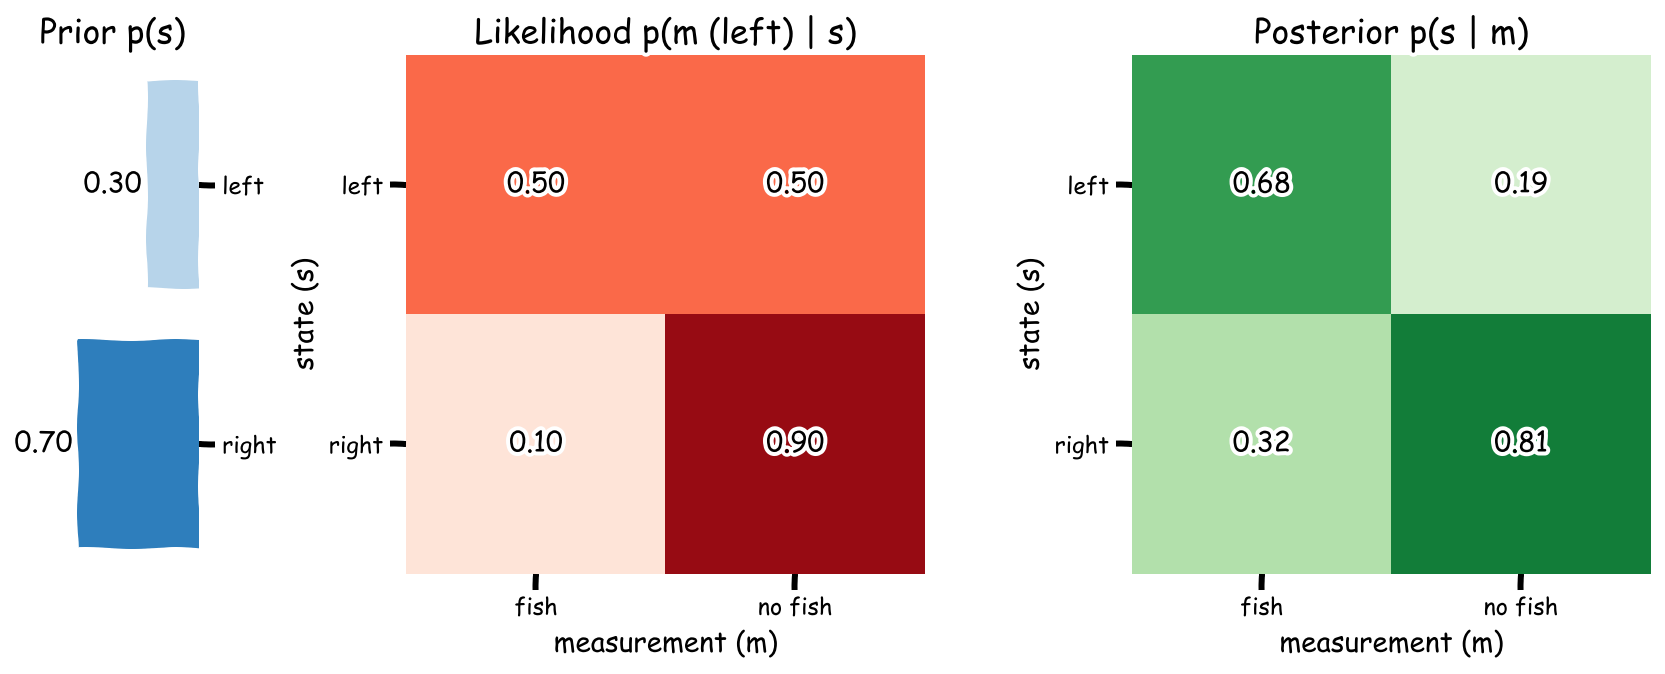
\includegraphics[scale=0.12]{Figures/BD/BD_Figure3.png}

 
\end{subbox}

\begin{subbox}{subbox}{Making Bayesian fishing decisions}
\scriptsize
We consider the expected utility of an action based on our belief (the posterior distribution) about where we think the fish are. Now we have all the components of a Bayesian decision: our prior information, the likelihood given a measurement, the posterior distribution (belief) and our utility (the gains and losses). This allows us to consider the relationship between the true value of the hidden state, $s$, and what we \textit{expect} to get if we take action, $a$, based on our belief!


\centering
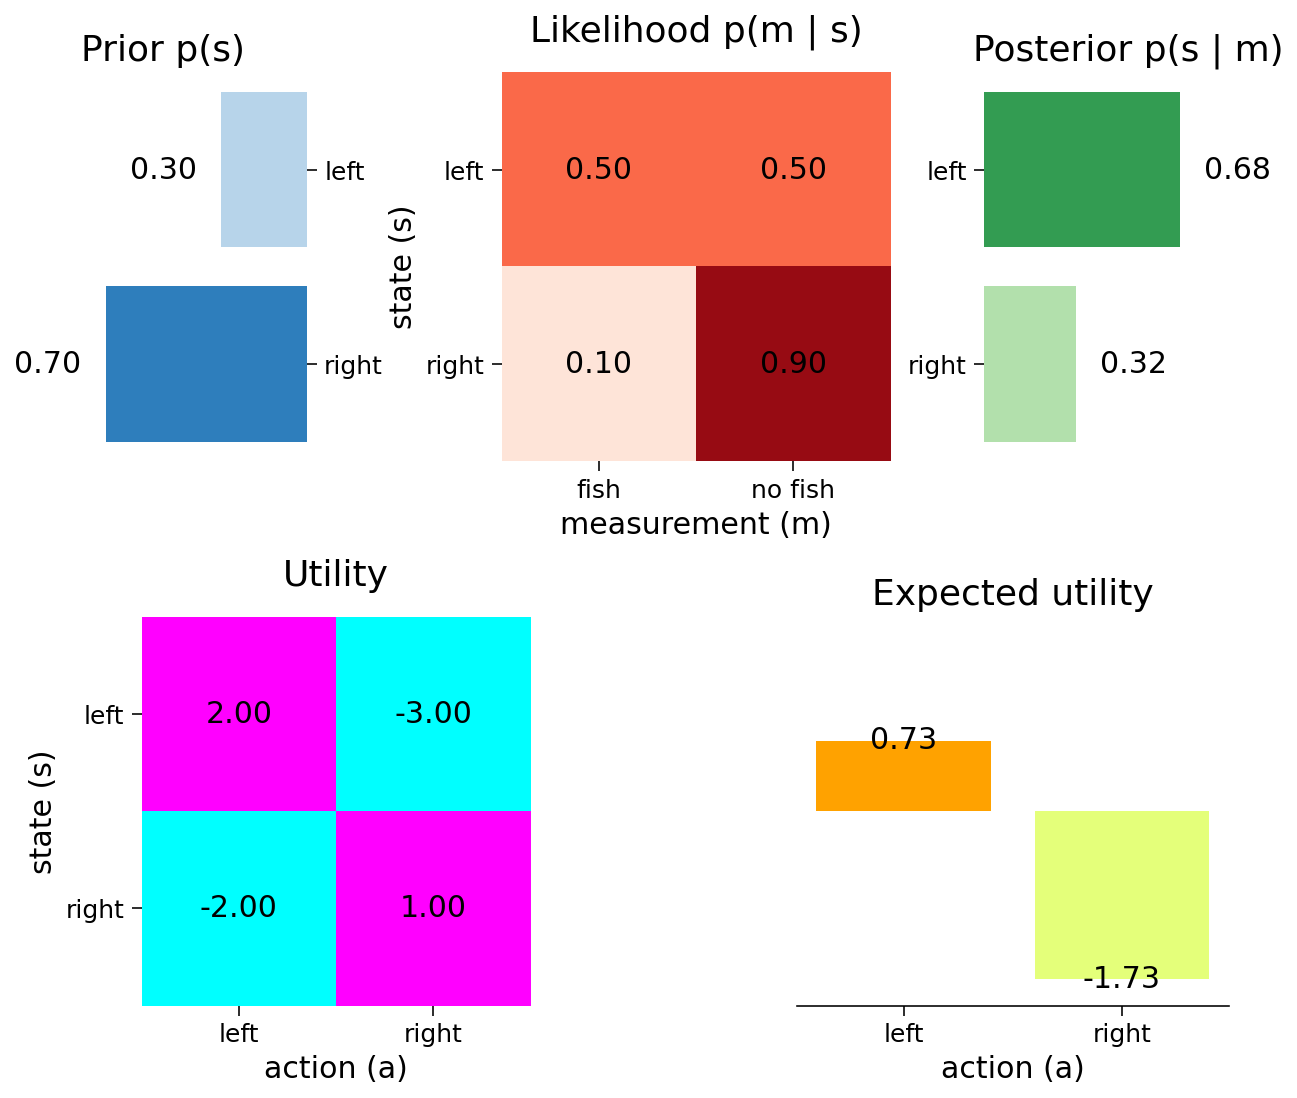
\includegraphics[scale=0.25]{Figures/BD/BD_Figure4.png}

 
\end{subbox}
\end{textbox}
%%%%%%%%%%%%%%%%%%%%%%%%%%%%%%%%%%%%%%%%%%%%%%%%%%
%%%%%%%%%%%%%%%%%%%%%%%%%%%%%%%%%%%%%%%%%%%%%%%%%%
%%% TUTORIAL 2
%%%%%%%%%%%%%%%%%%%%%%%%%%%%%%%%%%%%%%%%%%%%%%%%%%
%%%%%%%%%%%%%%%%%%%%%%%%%%%%%%%%%%%%%%%%%%%%%%%%%%
\begin{textbox}{\href{https://compneuro.neuromatch.io/tutorials/W3D1_BayesianDecisions/student/W3D1_Tutorial2.html}{Bayesian inference and decisions with continuous hidden state } }
\begin{subbox}{subbox}{Astrocat!}
\scriptsize
Let's say you are a cat astronaut - Astrocat! You are navigating around space using a jetpack and your goal is to chase a mouse. 

Since you are a cat, you don't have opposable thumbs and cannot control your own jet pack. It can only be controlled by ground control back on Earth. 

For them to be able to guide you, they need to know where you are. They are trying to figure out your location. They have prior knowledge of your location - they know you like to hang out near the space mouse. They can also get an unreliable quick glimpse: they are taking a measurement of the hidden state of your location.

They will try to figure out your location using Bayes rule and Bayesian decisions - as we will see throughout this tutorial.


\begin{center}
    
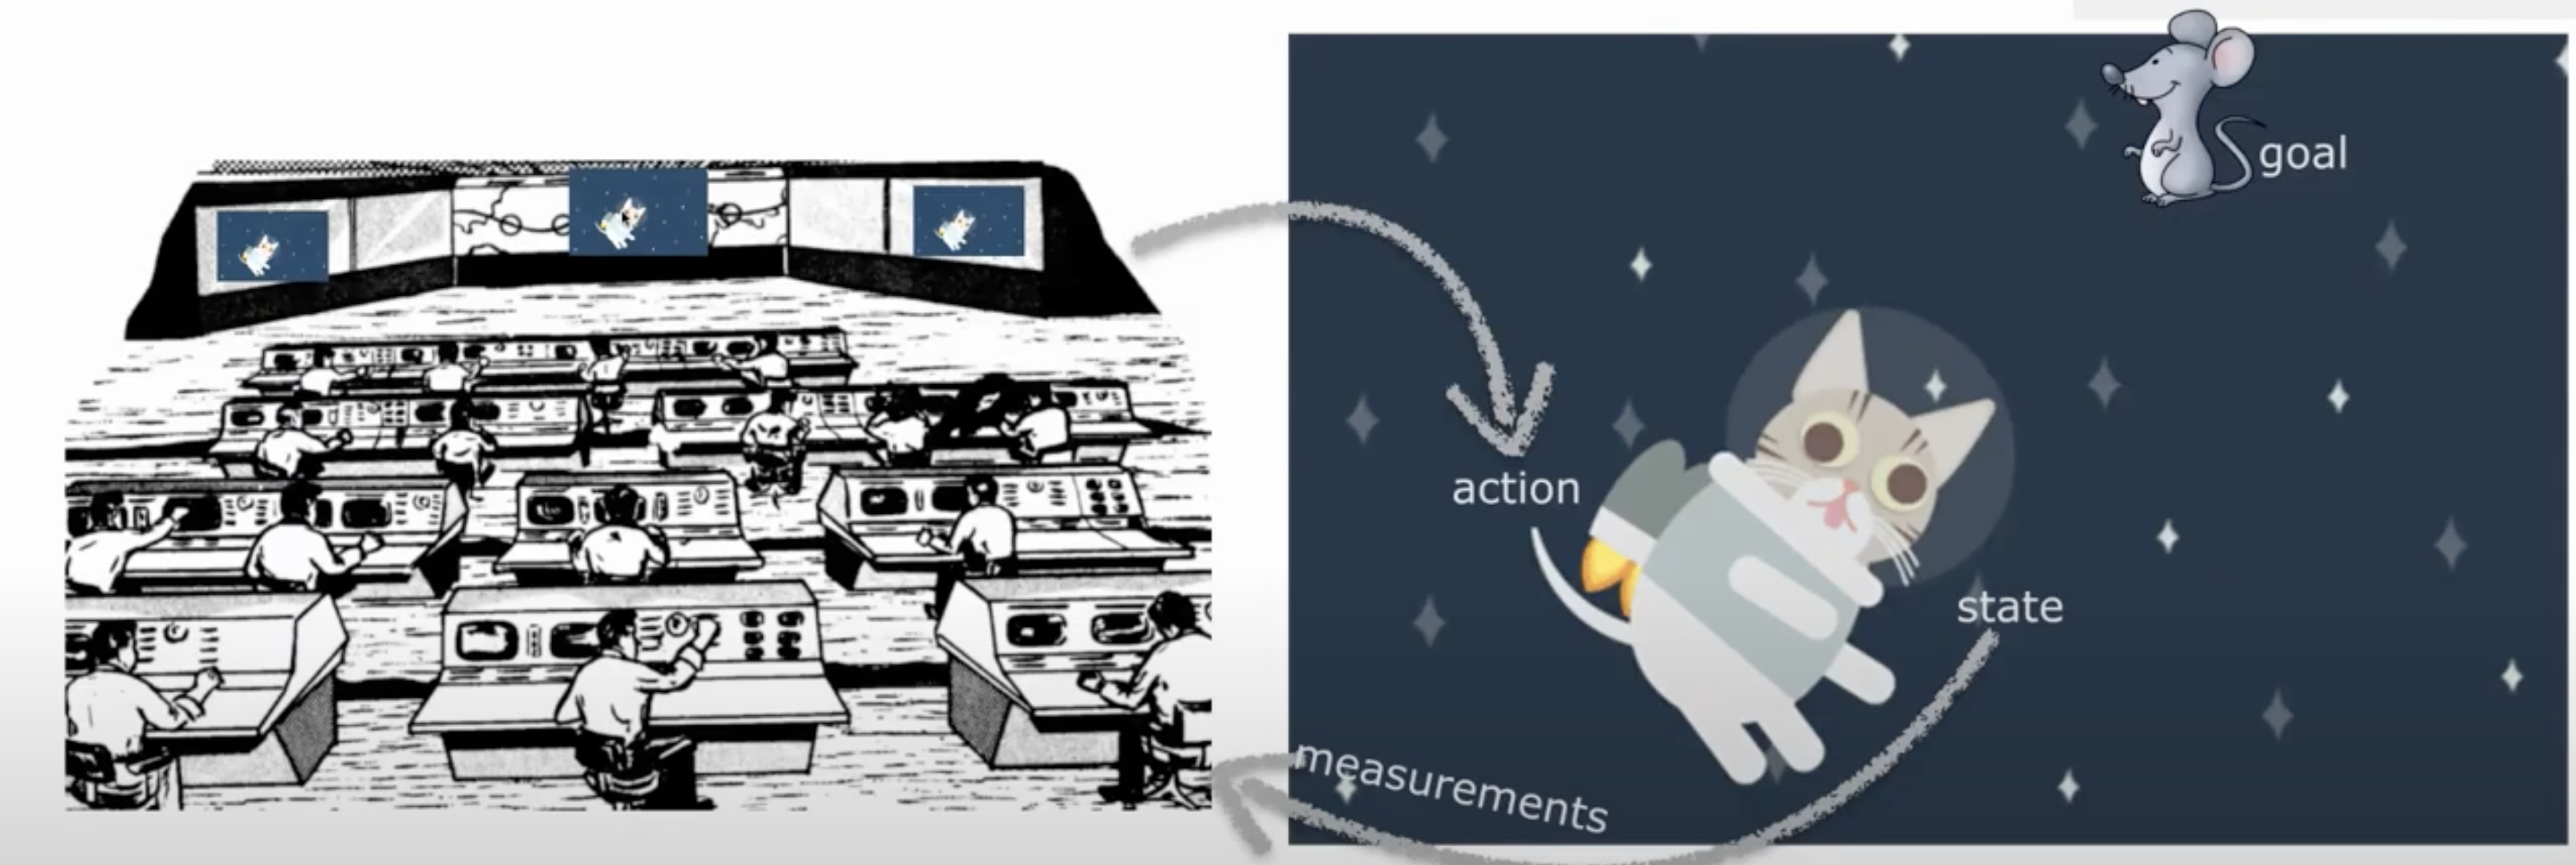
\includegraphics[scale=0.1]{Figures/BD/BD_Figure5.png}
\end{center}


Astrocat is in space and we are considering the position along one dimension. So, the hidden state, s, is the true location. The satellites represent potential loss, and the space mouse, gain. Using indirect measurements, you as ground control, can estimate where Astrocat is or decide where it's likely better to send Astrocat.

Remember, in this example, you can think of yourself as a scientist trying to decide where we believe Astrocat is, how to select a point estimate (single guess of location) based on possible errors, and how to account for the uncertainty we have about the location of the satellite and the space mouse. In fact, this is the kind of problem real scientists working to control remote satellites face! However, we can also think of this as what your brain does when it wants to determine a target to make a movement or hit a tennis ball! A number of classic experiments use this kind of framing to study how *optimal* human decisions or movements are! Some examples are in the further reading document.

\end{subbox}

\begin{subbox}{subbox}{Probability distribution of Astrocat location}
\scriptsize
We are going to think first about how Ground Control should estimate his position. We won't consider measurements yet, just how to represent the uncertainty we might have in general. We are now dealing with a continuous distribution - Astrocat's location can be any real number. In the last tutorial, we were dealing with a discrete distribution - the fish were either on one side or the other. 

So how do we represent the probability of each possible point (an infinite number) where the Astrocat could be? 
The Bayesian approach can be used on any probability distribution. While many variables in the world require representation using complex or unknown (e.g. empirical) distributions, we will be using the Gaussian distributions or extensions of it.

\end{subbox}
\end{textbox}
%%%%%%%%%%%%%%%%%%%%%%%%%%%%%%%%%%%%%%%%%%%%%%%%%%
%%%%%%%%%%%%%%%%%%%%%%%%%%%%%%%%%%%%%%%%%%%%%%%%%%
\begin{textbox}{\href{https://compneuro.neuromatch.io/tutorials/W3D1_BayesianDecisions/student/W3D1_Tutorial2.html}{Bayesian inference and decisions with continuous hidden state } }
\begin{subbox}{subbox}{The Gaussian distribution}
\scriptsize
Tne distribution we will use throughout this tutorial is the \textbf{Gaussian distribution}, which is also sometimes called the normal distribution. 

This is a special, and commonly used, distribution for a couple reasons. It is actually the focus of one of the most important theorems in statistics: the Central Limit Theorem. This theorem tells us that if you sum a large number of samples of a variable, that sum is normally distributed \textit{no matter what} the original distribution over a variable was. This is a bit too in-depth for us to get into now but check out links in the Bonus for more information. Additionally, Gaussians have some really nice mathematical properties that permit simple closed-form solutions to several important problems. As we will see later in this tutorial, we can extend Gaussians to be even more flexible and well approximate other distributions using mixtures of Gaussians. In short, the Gaussian is probably the most important continuous distribution to understand and use.

Gaussians have two parameters. The \textbf{mean} $\mu$, which sets the location of its center. Its "scale" or spread is controlled by its \textbf{standard deviation} $\sigma$ or its square, the \textbf{variance} $\sigma^2$. These can be a bit easy to mix up: make sure you are careful about whether you are referring to/using standard deviation or variance.


The equation for a Gaussian distribution on a variable $x$ is:
\begin{equation}
\mathcal{N}(\mu,\sigma^2) = \frac{1}{\sqrt{2\pi\sigma^2}}\exp\left(\frac{-(x-\mu)^2}{2\sigma^2}\right)
\end{equation}

In our example, $x$ is the location of the Astrocat in one direction. $\mathcal{N}(\mu,\sigma^2)$ is a standard notation to refer to a $\mathcal{N}$ormal (Gaussian) distribution. For example, $\mathcal{N}(0, 1)$ denotes a Gaussian distribution with mean 0 and variance 1. 

\end{subbox}

\begin{subbox}{subbox}{Multiplying Gaussians}
\scriptsize
When we multiply Gaussians, we are not multiplying random variables but the actual underlying distributions. If we multiply two Gaussian distributions, with means $\mu_1$ and $\mu_2$ and standard deviations $\sigma_1$ and $\sigma_2$, we get another Gaussian. The Gaussian resulting from the multiplication will have mean $\mu_3$ and standard deviation $\sigma_3$ where:

\begin{align}
\mu_{3} &= a\mu_{1} + (1-a)\mu_{2} \\
\sigma_{3}^{-2} &= \sigma_{1}^{-2} + \sigma_{2}^{-2} \\
a &= \frac{\sigma_{1}^{-2}}{\sigma_{1}^{-2} + \sigma_{2}^{-2}}
\end{align}

This may look confusing but keep in mind that the information in a Gaussian is the inverse of its variance: $\frac{1}{\sigma^2}$. Basically, when multiplying Gaussians, the mean of the resulting Gaussian is a weighted average of the original means, where the weights are proportional to the amount of information of that Gaussian.

\end{subbox}
\end{textbox}
%%%%%%%%%%%%%%%%%%%%%%%%%%%%%%%%%%%%%%%%%%%%%%%%%%
%%%%%%%%%%%%%%%%%%%%%%%%%%%%%%%%%%%%%%%%%%%%%%%%%%
\begin{textbox}{\href{https://compneuro.neuromatch.io/tutorials/W3D1_BayesianDecisions/student/W3D1_Tutorial2.html}{Bayesian inference and decisions with continuous hidden state } }
\begin{subbox}{subbox}{Multiplying Gaussians}
\scriptsize

Multiplying two Gaussians, imagine we want to find the middle location between the satellite and the space mouse. This would be the center (average) of the two locations. Because we have uncertainty, we need to weigh our uncertainty in thinking about the most likely place. 


\begin{center}
    
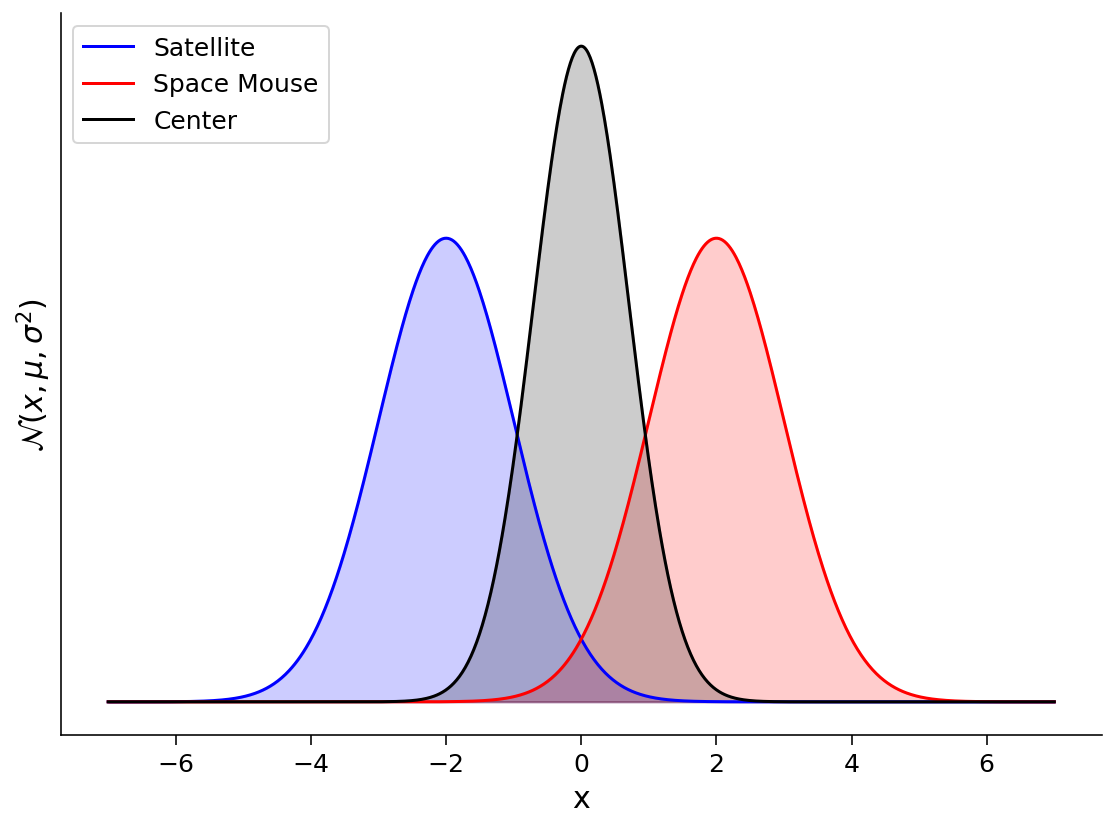
\includegraphics[scale=0.18]{Figures/BD/BD_Figure6.png}
\end{center}
\end{subbox}
\begin{subbox}{subbox}{Mixtures of Gaussians}
\scriptsize

What if our continuous distribution isn't well described by a single bump? For example, what if the Astrocat is often either in one place or another - a Gaussian distribution would not capture this well! We need a multimodal distribution. Luckily, we can extend Gaussians into a \textit{mixture of Gaussians}, which are more complex distributions.  

In a Gaussian mixture distribution, you are essentially adding two or more weighted standard Gaussian distributions (and then normalizing so everything integrates to 1). Each standard Gaussian involved is described, as normal, by its mean and standard deviation. Additional parameters in a mixture of Gaussians are the weights you put on each Gaussian (π). The following demo should help clarify how a mixture of Gaussians relates to the standard Gaussian components. We will not cover the derivation here but you can work it out as a bonus exercise.

Mixture distributions are a common tool in Bayesian modeling and an important tool in general.

We will examining a mixture of two Gaussians. We will have one weighting parameter, $\pi$, that tells us how to weigh one of the Gaussians. The other is weighted by $1 -\pi$. 

\begin{center}
    
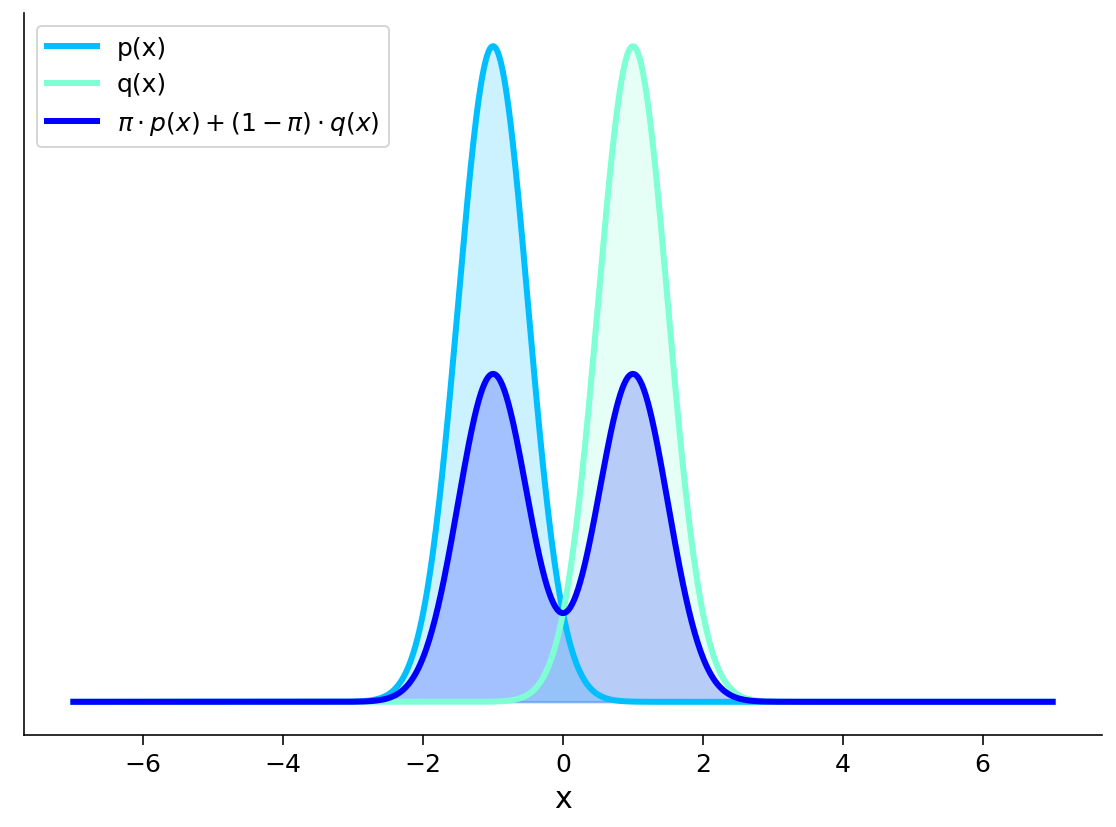
\includegraphics[scale=0.22]{Figures/BD/BD_Figure7.png}
\end{center}
\end{subbox}


\end{textbox}
%%%%%%%%%%%%%%%%%%%%%%%%%%%%%%%%%%%%%%%%%%%%%%%%%%
%%%%%%%%%%%%%%%%%%%%%%%%%%%%%%%%%%%%%%%%%%%%%%%%%%
\begin{textbox}{\href{https://compneuro.neuromatch.io/tutorials/W3D1_BayesianDecisions/student/W3D1_Tutorial2.html}{Bayesian inference and decisions with continuous hidden state } }
\begin{subbox}{subbox}{Utility Loss Estimators}
\scriptsize

There are lots of different possible loss functions. We will focus on three: \textbf{mean-squared error} where the loss is the difference between truth and estimate squared, \textbf{absolute error} where the loss is the absolute difference between truth and estimate, and \textbf{Zero-one Loss} where the loss is 1 unless we're exactly right (the estimate equals the truth). We can represent these with the following formulas:

\begin{eqnarray}
\textrm{Mean Squared Error} &=& (\mu - \hat{\mu})^2 \\ 
\textrm{Absolute Error} &=& \big|\mu - \hat{\mu}\big| \\ 
\textrm{Zero-One Loss} &=& \begin{cases}
                            0,& \textrm{if } \mu = \hat{\mu} \\
                            1,              & \textrm{otherwise}
                            \end{cases}
\end{eqnarray}


We will now explore how these different loss functions change our expected utility!

\begin{center}
    
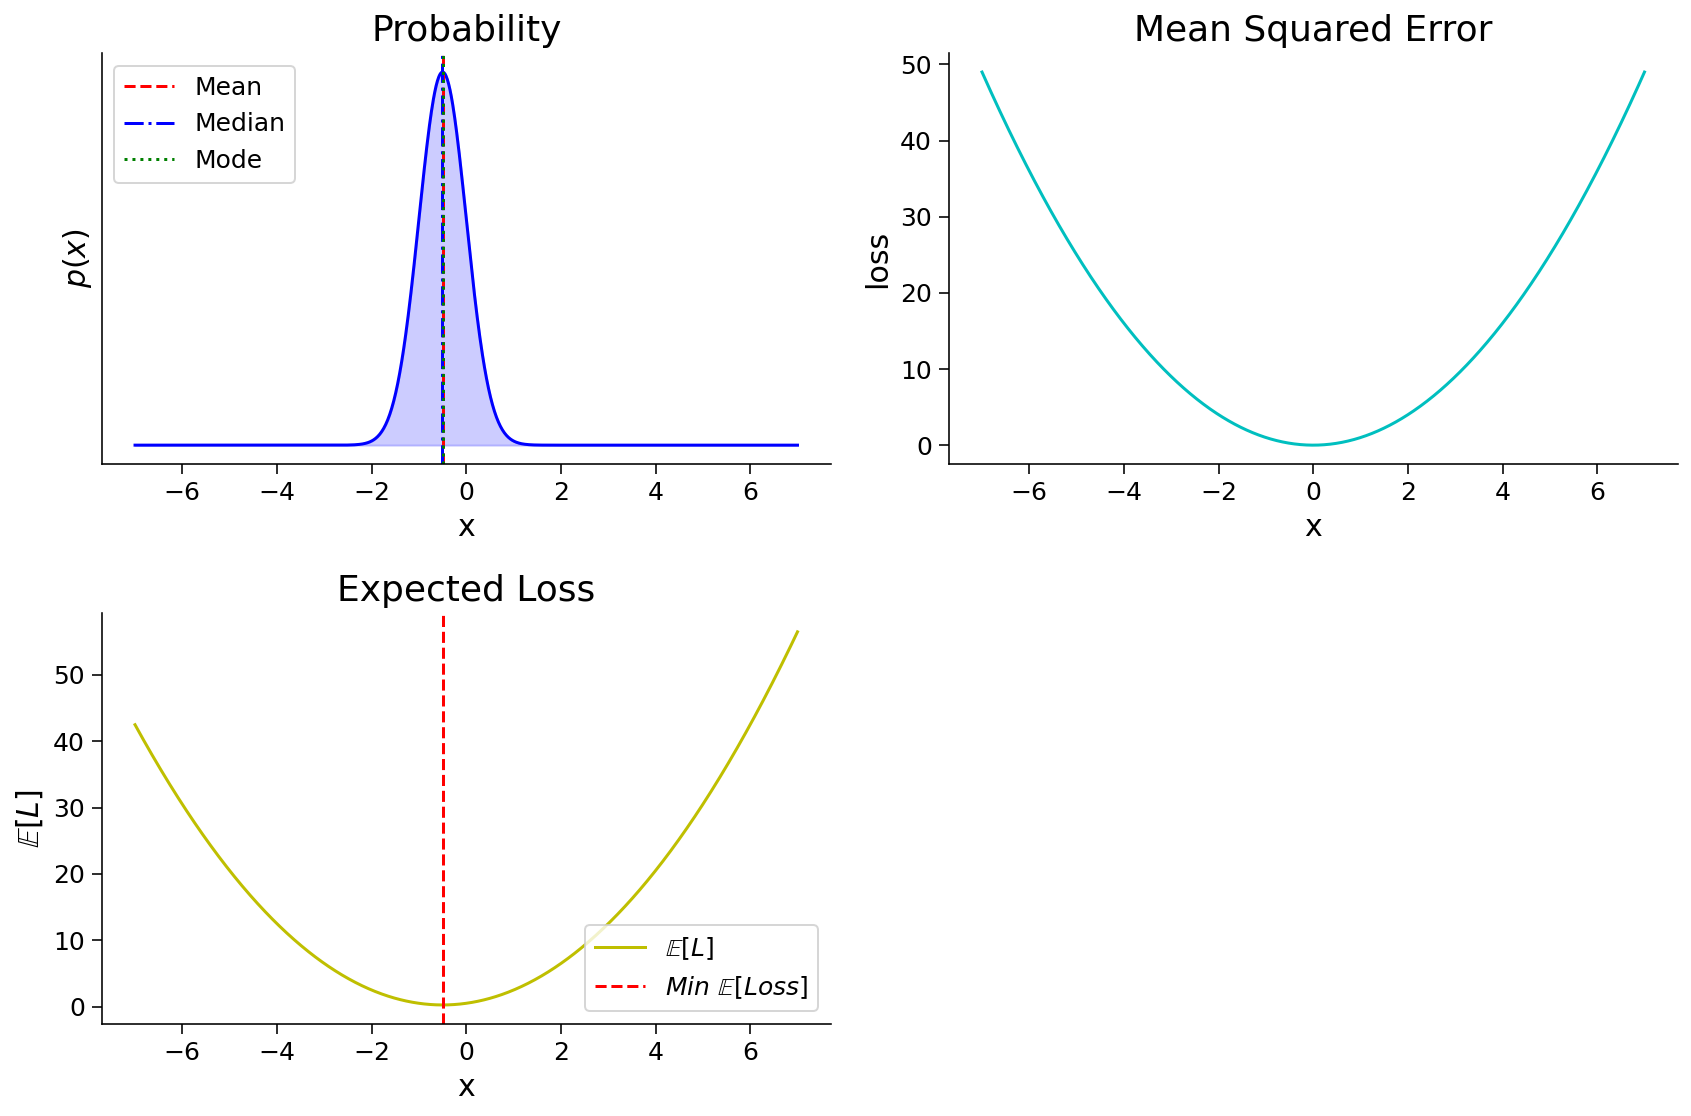
\includegraphics[scale=0.22]{Figures/BD/BD_Figure8.png}
\end{center}

You can see that what coordinates you would provide for Astrocat aren't necessarily easy to guess just from the probability distribution. You need the concept of utility/loss and a specific loss function to determine what estimate you should give.

For symmetric distributions, you will find that the mean, median and mode are the same. However, for distributions with \textit{skew}, like the Gamma distribution or the Exponential distribution, these will be different. You will be able to explore more distributions as priors below.

\end{subbox}

\end{textbox}
%%%%%%%%%%%%%%%%%%%%%%%%%%%%%%%%%%%%%%%%%%%%%%%%%%
%%%%%%%%%%%%%%%%%%%%%%%%%%%%%%%%%%%%%%%%%%%%%%%%%%
\begin{textbox}{\href{https://compneuro.neuromatch.io/tutorials/W3D1_BayesianDecisions/student/W3D1_Tutorial2.html}{Bayesian inference and decisions with continuous hidden state } }
\begin{subbox}{subbox}{A more complex loss function}
\scriptsize



The loss functions we just explored were fairly simple and are often used. However, life can be complicated and in this case, Astrocat cares about both being near the space mouse and avoiding the satellites. This means we need a more complex loss function that captures this! 

We know that we want to estimate Astrocat to be closer to the mouse, which is safe and desirable, but further away from the satellites, which is dangerous! So, rather than thinking about the *Loss* function, we will consider a generalized utility function that considers gains and losses that \textit{matter} to Astrocat!
\begin{center}
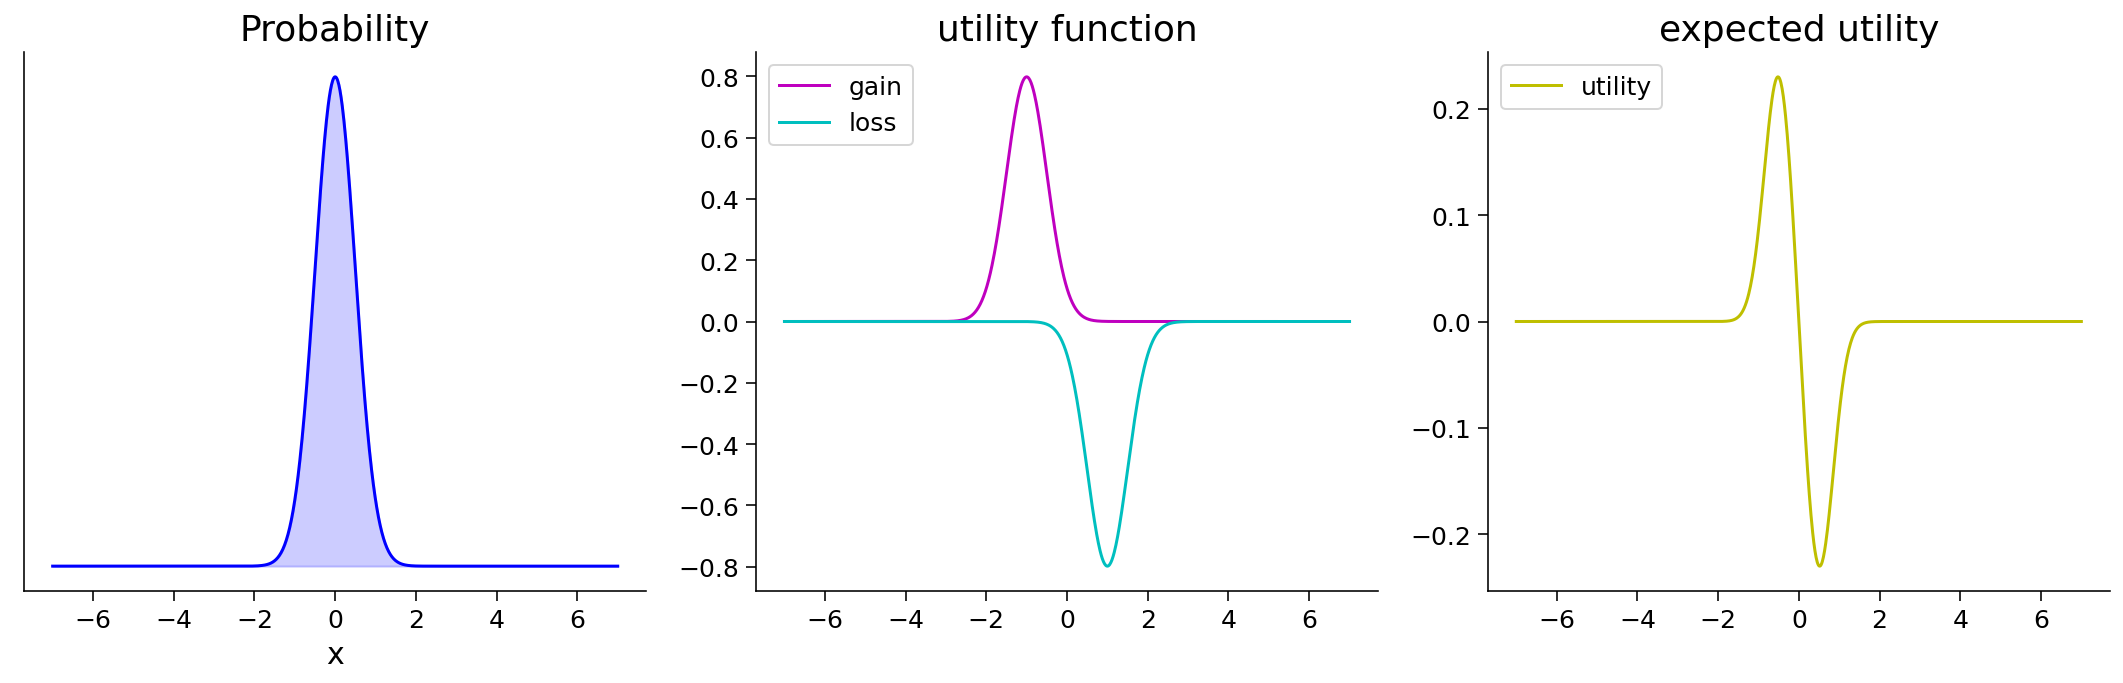
\includegraphics[scale=0.18]{Figures/BD/BD_Figure9.png}
\end{center}


\end{subbox}
\begin{subbox}{subbox}{Correlation and marginalization}
\scriptsize

If the two variables in a two dimensional Gaussian are independent, looking at one tells us nothing about the other. But what if the the two variables are correlated (covary)?

The covariance of two Gaussians with means $\mu_X$ and $\mu_Y$ and standard deviations $\sigma_X$ and $\sigma_Y$is:

\begin{equation}
\sigma_{XY} = \mathbb{E}[(X-\mu_{X})(Y-\mu_{Y})]
\end{equation}

$\mathbb{E}[\cdot]$ here denotes the expected value. So the covariance is the expected value of the random variable $X$ minus the mean of the Gaussian distribution on $X$ times the random variable Y minus the mean of the Gaussian distribution on $Y$.

The correlation is the covariance normalized, so that it goes between -1 (exactly anticorrelated) to 1 (exactly correlated).

\begin{equation}
\rho_{XY} = \frac{\sigma_{XY}}{\sigma_{X}\sigma_{Y}}
\end{equation}

These are key concepts and while we are considering two hidden states (or two random variables), they extend to $N$ dimensional vectors of Gaussian random variables. You will find these used all over computational neuroscience.
\begin{center}
    
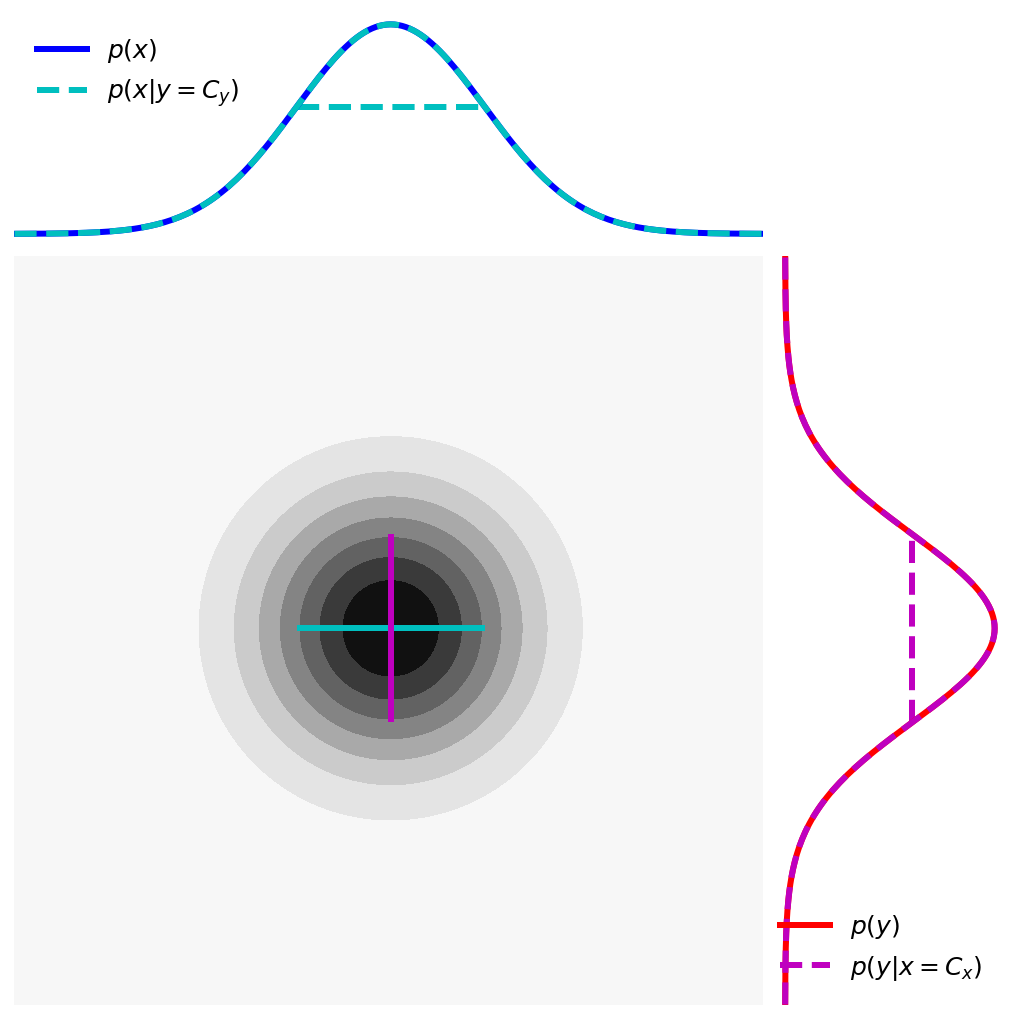
\includegraphics[scale=0.18]{Figures/BD/BD_Figure10.png}
\end{center}

\end{subbox}
\end{textbox}
%%%%%%%%%%%%%%%%%%%%%%%%%%%%%%%%%%%%%%%%%%%%%%%%%%
%%%%%%%%%%%%%%%%%%%%%%%%%%%%%%%%%%%%%%%%%%%%%%%%%%
\begin{textbox}{\href{https://compneuro.neuromatch.io/tutorials/W3D1_BayesianDecisions/student/W3D1_Tutorial2.html}{Bayesian inference and decisions with continuous hidden state } }
\begin{subbox}{subbox}{Bayes' theorem for continuous distributions}
\scriptsize

The continuous case allows us to consider how the shape of the posterior distribution can differ from the prior. The Gaussian case is the most fundamental, but asymmetric priors (or likelihoods) and posteriors allow us to see how the mean, median and mode can be affected differently when we apply Bayes' theorem.

\end{subbox}
\begin{subbox}{subbox}{The Gaussian example}
\scriptsize
Bayes' rule tells us how to combine two sources of information: the prior (e.g., a noisy representation of Ground Control's expectations about where Astrocat is) and the likelihood (e.g., a noisy representation of the Astrocat after taking a measurement), to obtain a posterior distribution (our belief distribution) taking into account both pieces of information. Remember Bayes' rule:

\begin{equation}
\text{Posterior} = \frac{ \text{Likelihood} \times \text{Prior}}{ \text{Normalization constant}}
\end{equation}

We will look at what happens when both the prior and likelihood are Gaussians. In these equations, $\mathcal{N}(\mu,\sigma^2)$ denotes a Gaussian distribution with parameters $\mu$ and $\sigma^2$:

\begin{equation}
\mathcal{N}(\mu, \sigma) = \frac{1}{\sqrt{2 \pi \sigma^2}} \; \exp \bigg( \frac{-(x-\mu)^2}{2\sigma^2} \bigg)
\end{equation}

When both the prior and likelihood are Gaussians, Bayes Rule translates into the following form:
\tiny
\begin{align*}
\text{Likelihood} &= \mathcal{N}(\mu_{likelihood},\sigma_{likelihood}^2) \\
\text{Prior} &= \mathcal{N}(\mu_{prior},\sigma_{prior}^2) \\
\text{Posterior} &= \mathcal{N}\left( \frac{\sigma^2_{likelihood}\mu_{prior}+\sigma^2_{prior}\mu_{likelihood}}{\sigma^2_{likelihood}+\sigma^2_{prior}},\right.\\
& \left. \frac{\sigma^2_{likelihood}\sigma^2_{prior}}{\sigma^2_{likelihood}+\sigma^2_{prior}} \right) \\
&\propto \mathcal{N}(\mu_{likelihood},\sigma_{likelihood}^2) \times \mathcal{N}(\mu_{prior},\sigma_{prior}^2)
\end{align*}


\begin{center}
    
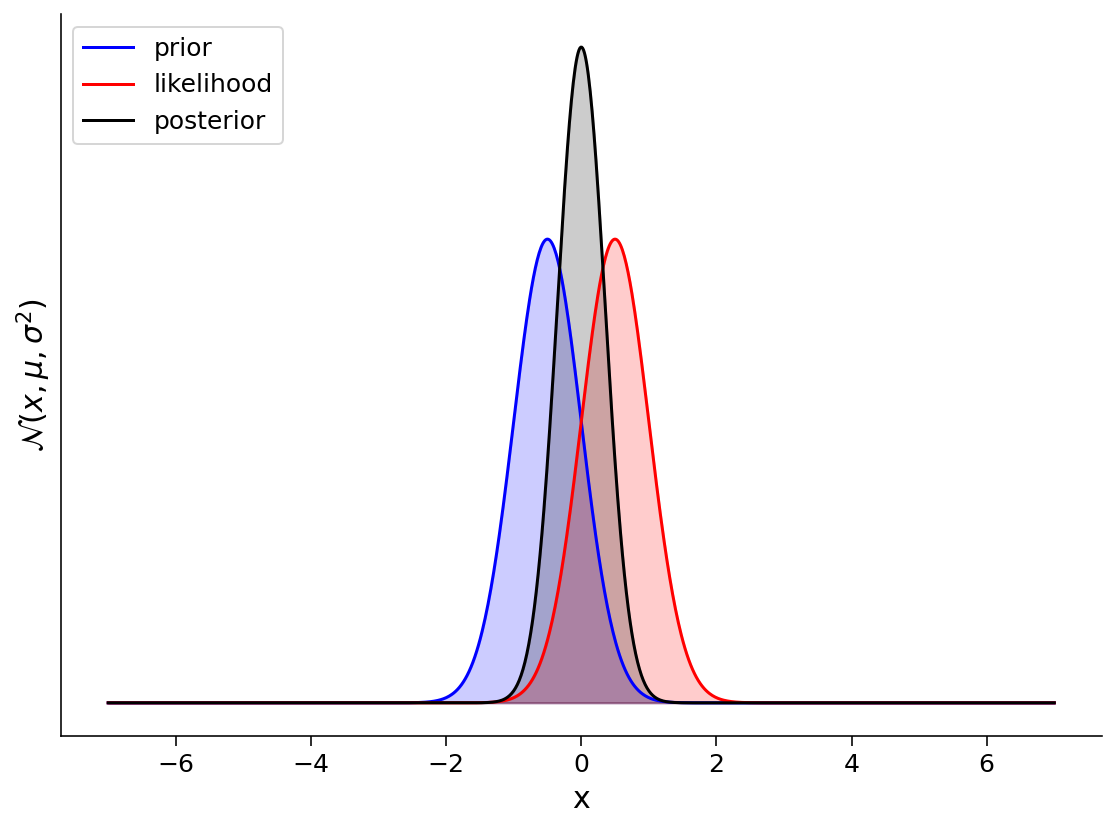
\includegraphics[scale=0.23]{Figures/BD/BD_Figure11.png}
\end{center}

\end{subbox}
\end{textbox}
%%%%%%%%%%%%%%%%%%%%%%%%%%%%%%%%%%%%%%%%%%%%%%%%%%
%%%%%%%%%%%%%%%%%%%%%%%%%%%%%%%%%%%%%%%%%%%%%%%%%%
\begin{textbox}{\href{https://compneuro.neuromatch.io/tutorials/W3D1_BayesianDecisions/student/W3D1_Tutorial2.html}{Bayesian inference and decisions with continuous hidden state } }
\begin{subbox}{subbox}{Bayesian estimation on the posterior}
\scriptsize


Bayesian decisions in continuous dimensions are the same as for the binary case. The only difference is that now, our Expected Utility is calculated using an integral and all of our probability distributions are continuous.
\begin{center}
    
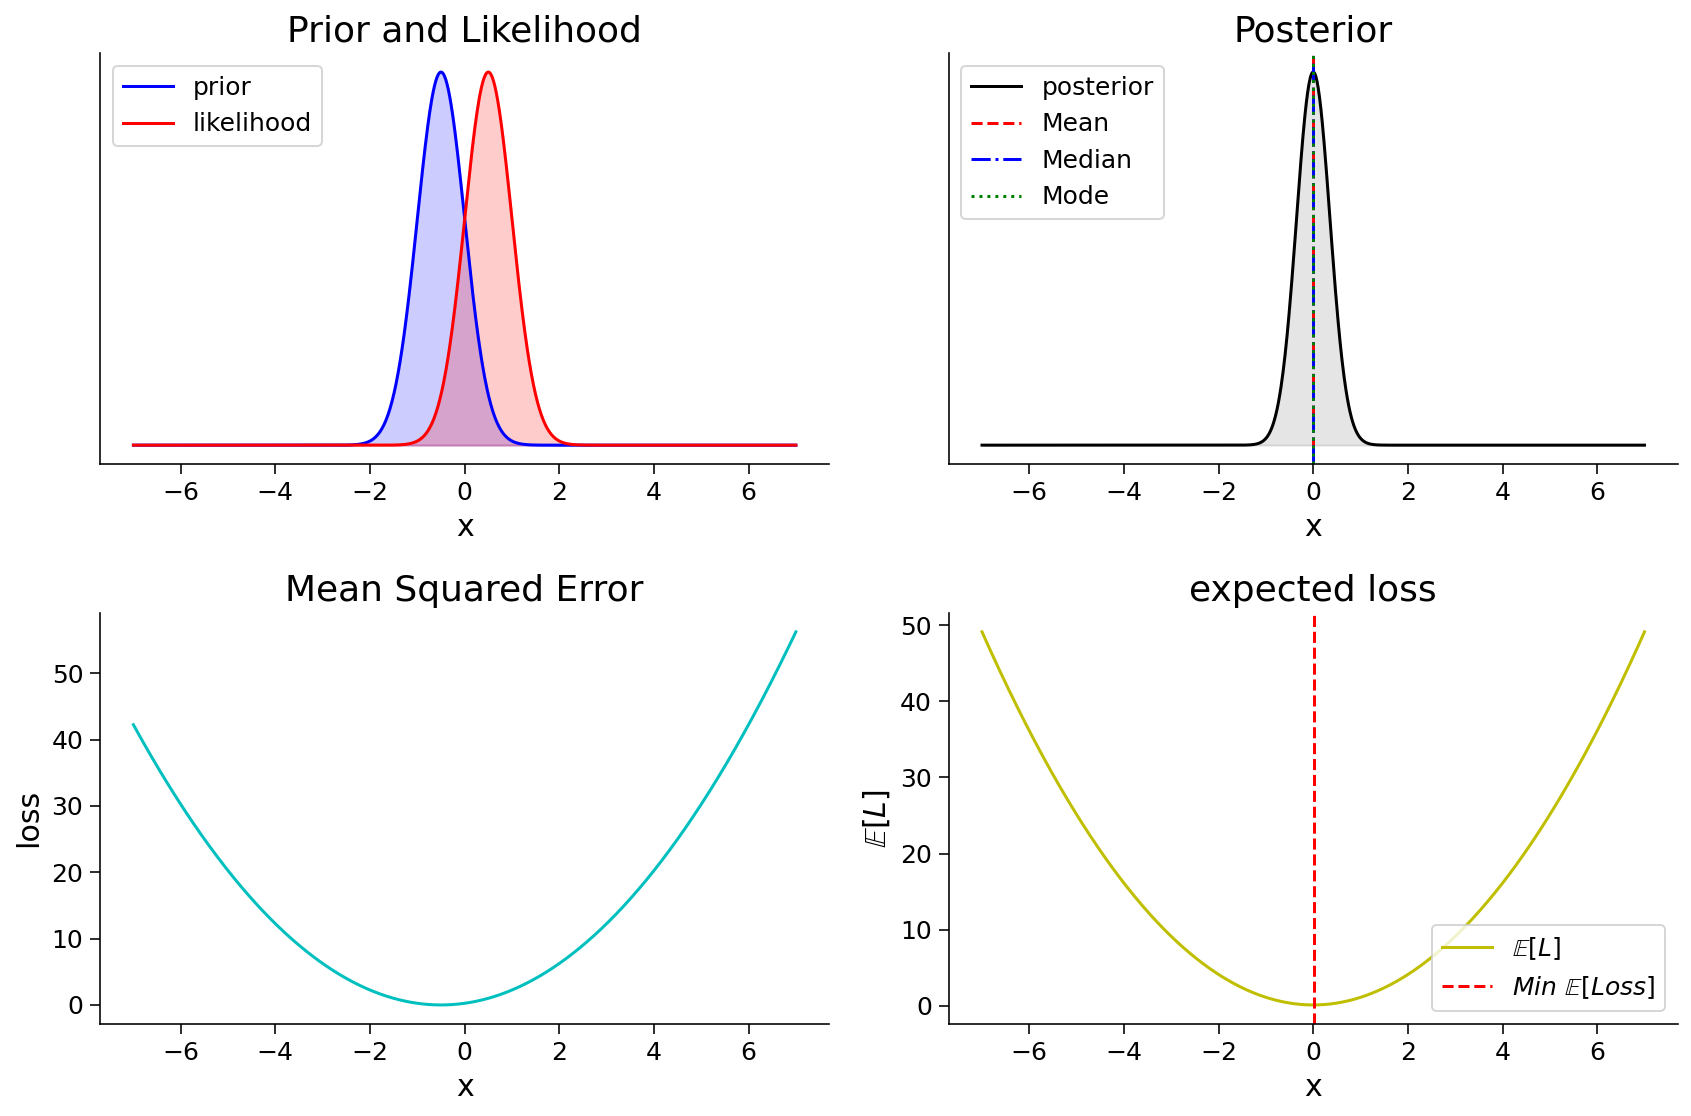
\includegraphics[scale=0.23]{Figures/BD/BD_Figure12.png}
\end{center}
\end{subbox}
\begin{subbox}{subbox}{Bayesian decisions}
\scriptsize
Finally, we can combine everything we have learned so far! 

Now, let's imagine we have just received a new measurement of Astrocat's location. We need to think about how we want to decide where Astrocat is, so that we can decide how far to tell Astrocat to move. However, we want to account for the satellite and Space Mouse location in this estimation. If we make an error towards the satellite, it's worse than towards Space Mouse. So, we will use our more complex utility function than before. 

\begin{center}
    
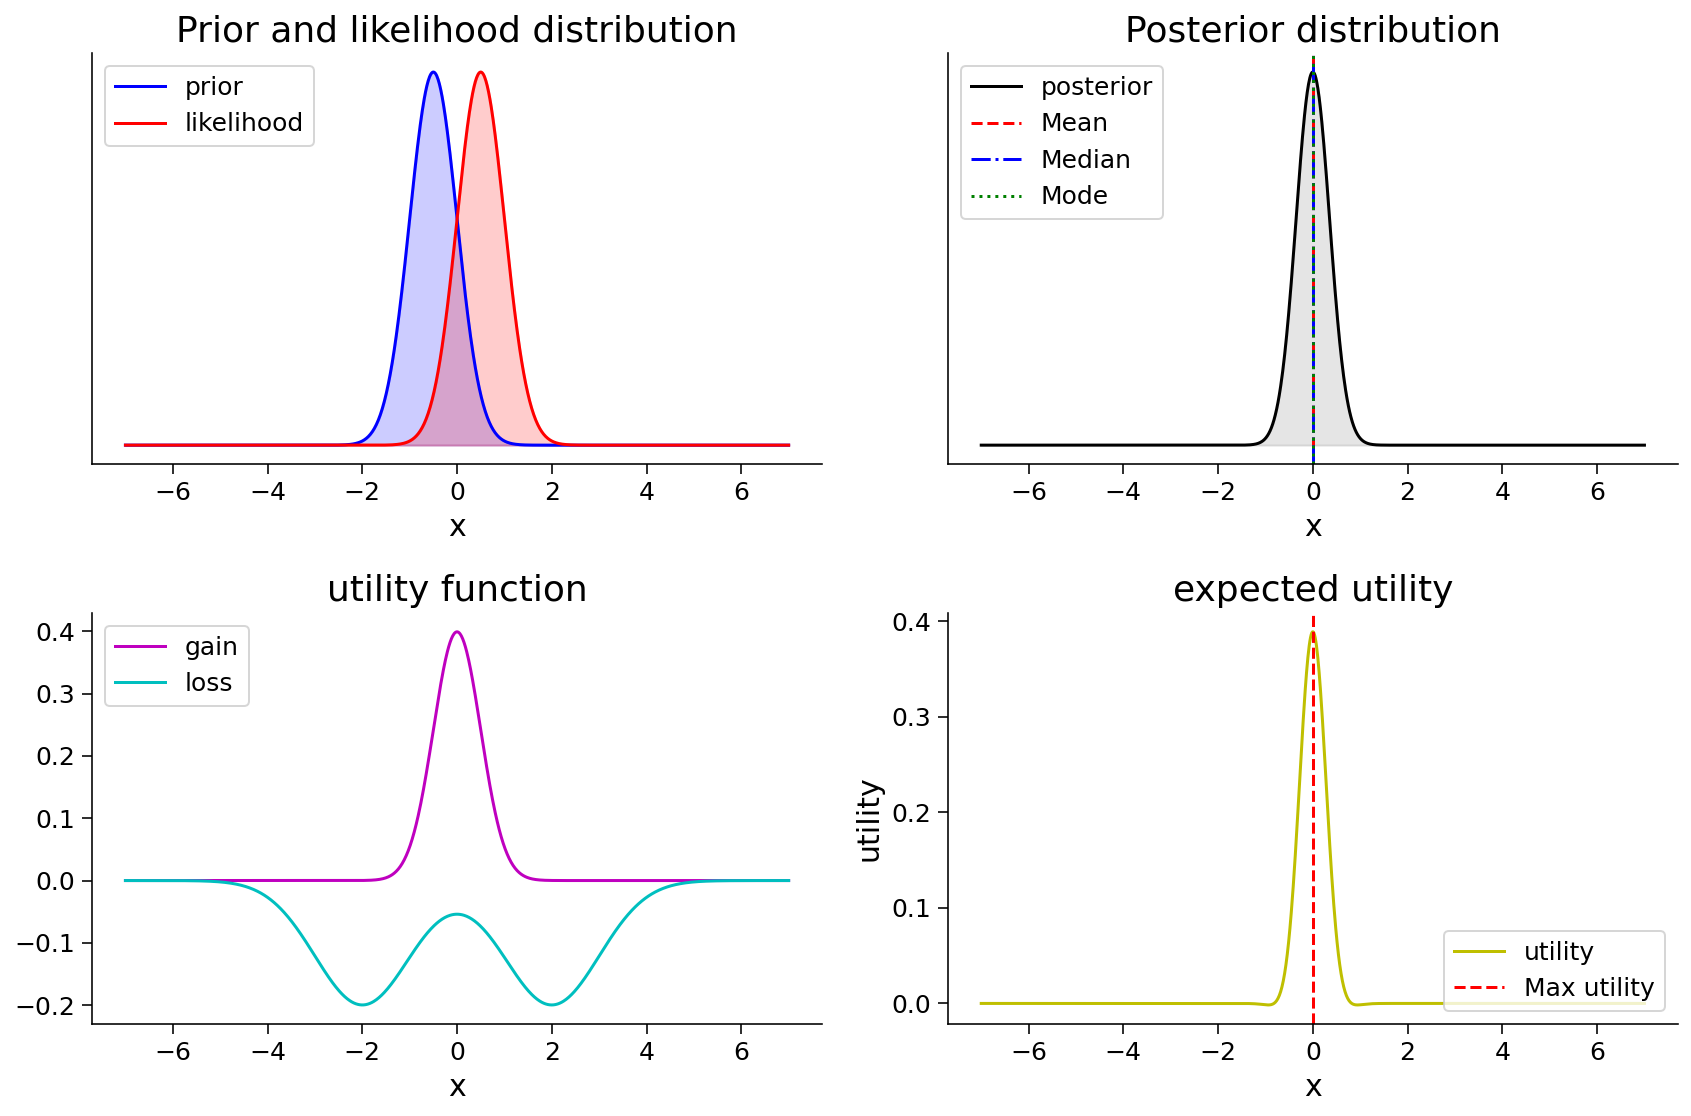
\includegraphics[scale=0.23]{Figures/BD/BD_Figure13.png}
\end{center}

\end{subbox}
\end{textbox}

